\documentclass[../main/thesis.tex]{subfiles}

\begin{document}

\section{Forecast verification metrics}
A robust verification scheme is essential to gain insight into how the developed forecasting product performs. Both from the point of view of a  developer which aim to increase the skill of the prediction but also from the user which may utilize the verification score to assess the quality of a given forecast \cite{Casati2008}. In the context of Sea Ice forecasting, a spatial field of continuos or discrete sea ice concentration is predicted, the latter being the case for the current work. Given the uneven distribution intra sea ice concentration classes as well as sea ice compared to ice free open water, simply comparing pixels for correctness would be biased by the large portion of open water and result in difficult to interpret values devoid of physical reasoning. \todo{Syk udokumentert påstand, må modereres} Furthermore, as the rate of maritime activity such as commercial shipping increases in the Arctic due to the sea ice decline \cite{Ho2010}, having user relevant metrics can aid and alleviate the risks surrounding Arctic navigation. As such, several studies have proposed calculating the position of the ice edge as a user relevant metric which also provides information of the distribution of the Sea Ice Concentration \cite{Dukhovskoy2015,Goessling2016,Goessling2018}. However, there is no agreement with how to best calculate the position of the Ice Edge, with the currently available metrics posing different advantages/disadvantages \cite{Palerme2019,Melsom2019}. For the purpose of this thesis, The ice edge position and length will be calculated according to \cite[Melsom 2019 et.al]{Melsom2019}, whereas the IIEE originally proposed by Goessling. H. \cite{Goessling2016} will also be utilized.

\subsection{Defining the Ice Edge}
\label{sec:iceedgelength}
The ice edge for a given Sea Ice Concentration product is derived on a per pixel basis, and defined as the grid cells which meet the condition

\begin{equation}
    \label{eq:iceedge}
    c[i,j] \geq c_q \wedge \text{min}{(c[i-1,j],c[i+1,j],c[i,j-1],c[i,j+1])} < c_e
\end{equation}

i.e. a pixel is marked as a ice edge pixel if the current pixel itself is larger than some given concentration threshold $c_e$ and the minimum of the pixel's 4-neighbors is less than the same threshold. Following this notation, E is defined as the set of grid cells which constitutes the ice edge \cite{Melsom2019}. Moreover, the marked grid cells each contribute to the total length of the ice edge, with each pixel's length contribution determined based on the number neighbors also marked as an ice edge pixel. Consequently, a neighborless pixel is assumed to yield a contribution the length of the diagonal to the ice-edge ($l = \sqrt2s$) where s is the side length of the pixel. A pixel with one neighbor a contributes a mixed horizontal - diagonasl length $l = \frac{s + \sqrt2s}{2}$. Finally a pixel with two or more neighbors contributes with a pixel side-length $l = s$. The final length of the ice edge length then become 
\begin{equation}
    L = \sum_\text{e in E} l_c
\end{equation}
where E represent the set of pixels constituting the ice edge as previously mentioned \cite{Melsom2019}.

\subsection{Integrated Ice Edge Error}
The Integrated Ice Edge Length (IIEE) is an error metric which compares the forecast to some ground truth target \cite{Goessling2016}. The metric is defined as 
\begin{equation}
    \label{eq:IIEE}
    \text{IIEE} = \text{O} + \text{U}
\end{equation}
where 
\begin{equation}
    \label{eq:a_plus}
    \text{O} = \int_A\text{max}(c_f - c_t, 0)dA
\end{equation}
and
\begin{equation}
    \label{eq:a_minus}
    \text{U} = \int_A\text{max}(c_t - c_f, 0)dA
\end{equation}
with $c_t$ and $c_f$ being the target and forecast concentration respectively, attaining a value of $1$ if the concentration for a given pixel i above a set threshold, and 0 elsewhere. From the definition of the metric, it can be seen that the IIEE is a sum of the forecast overshoot and undershoot compared to the ground truth target. For the current work, the IIEE is an easily interpreted metric as it quantifies the total forecast error and reports on the error spatially.

As an additional remark, note that O the current implementation in Equation (\ref{eq:a_plus}) is given as an area with sidelength dA, and is computed as one product against some other product. Conversely, for this work subscripts f and t denote forecast and target respectively, with the directionality of the computations in Equation (\ref{eq:a_plus}) and (\ref{eq:a_minus}) indicating that the forecast is inspected with respect to the target. However, the metric can and has also been used to define the set of pixels which constitutes its area. To clearly distinguish between the area O and the set of pixels used to compute O, $A^+$ will be used to note the latter. Similarly, $A^-$ will represent the set of pixels constituting U. Finally, it can be seen that $A^+$ and $A^-$ represent the False Positive and False Negatives of the forecast respectively.

Furthermore, the IIEE can be combined with the length of the Ice Edge which was derived in the previous section \ref{sec:iceedgelength}. Thus, the metric is seasonally normalized, assuming that the IIEE and Ice Edge Length is seasonally correlated.

\section{Impact of increased resolution on the IIEE}
\label{sec:Impact of increased resolution on the IIEE}
From both the definition of Equation (\ref{eq:iceedge}) and (\ref{eq:IIEE}), it can be seen that there is a dependance on the number of pixels which constitutes the ice edge. However, what effect would a change of resolution, i.e. change in number of pixels, have on the IIEE / ice edge length ratio? To answer this question, the "two day" ice edge targets where compared against persistance on all valid two day forecasts samples for the period 2019 - 2021. Furthermore, the original target resolution of 1km will be assessed, as well as a regrided product downscaled onto a 10km resolution.

The Pearson correlation coefficient was computed directly from the DataFrames containing the metrics for both 1km and 10km resolution, using the statistical Python package Pandas \cite{reback2020pandas,mckinney-proc-scipy-2010}. For clarity, the correlation between mean\_length and IIEE for 1km and 10km was calculated. From the resulting computations, the correlation coefficient gets reported as $r_{mean\_length} = 0.9620$ and $r_{IIEE} = 0.9995$. Furthermore, the IIEE divided by the mean length correlation is reported as $r_{normalized\_IIEE} = 0.9667$. Finally, Figure (\ref{fig:normIIEE}) display the mean monthly IIEE computed along the inspected three year period.

By inspecting Figure (\ref{fig:normIIEE}) in conjunction with the reported correlation coefficients, it can be seen that increasing the working resolution of the dataset from 1km to 10km has a negligible impact on the reported metrics. Though the 1km ice edge is about $~2$ times longer than the 10km, coarser resolution ice edge, it does not impact the overall stability of the normalized IIEE metric. Moreover, the normalized IIEE is reduced for the 1km grid. This could be a consequence of each pixel's spatial extent covering less area. Note that the from the definition of the IIEE given in Equation (\ref{eq:IIEE}), the un-normalized metric is dependent on pixel spatial size. Thus, the number of pixels constituting the sum is inverse proportional with the size of each pixel, hence keeping the stability of the values. However, a discrepancy may arise due to the coarser resolution pixels covering a larger area, thus losing out on the fine details. However, for the current work, the ratio of 1km IIEE and 10km IIEE is $0.9938$, indicating that they are close to equal. 

\begin{figure}
    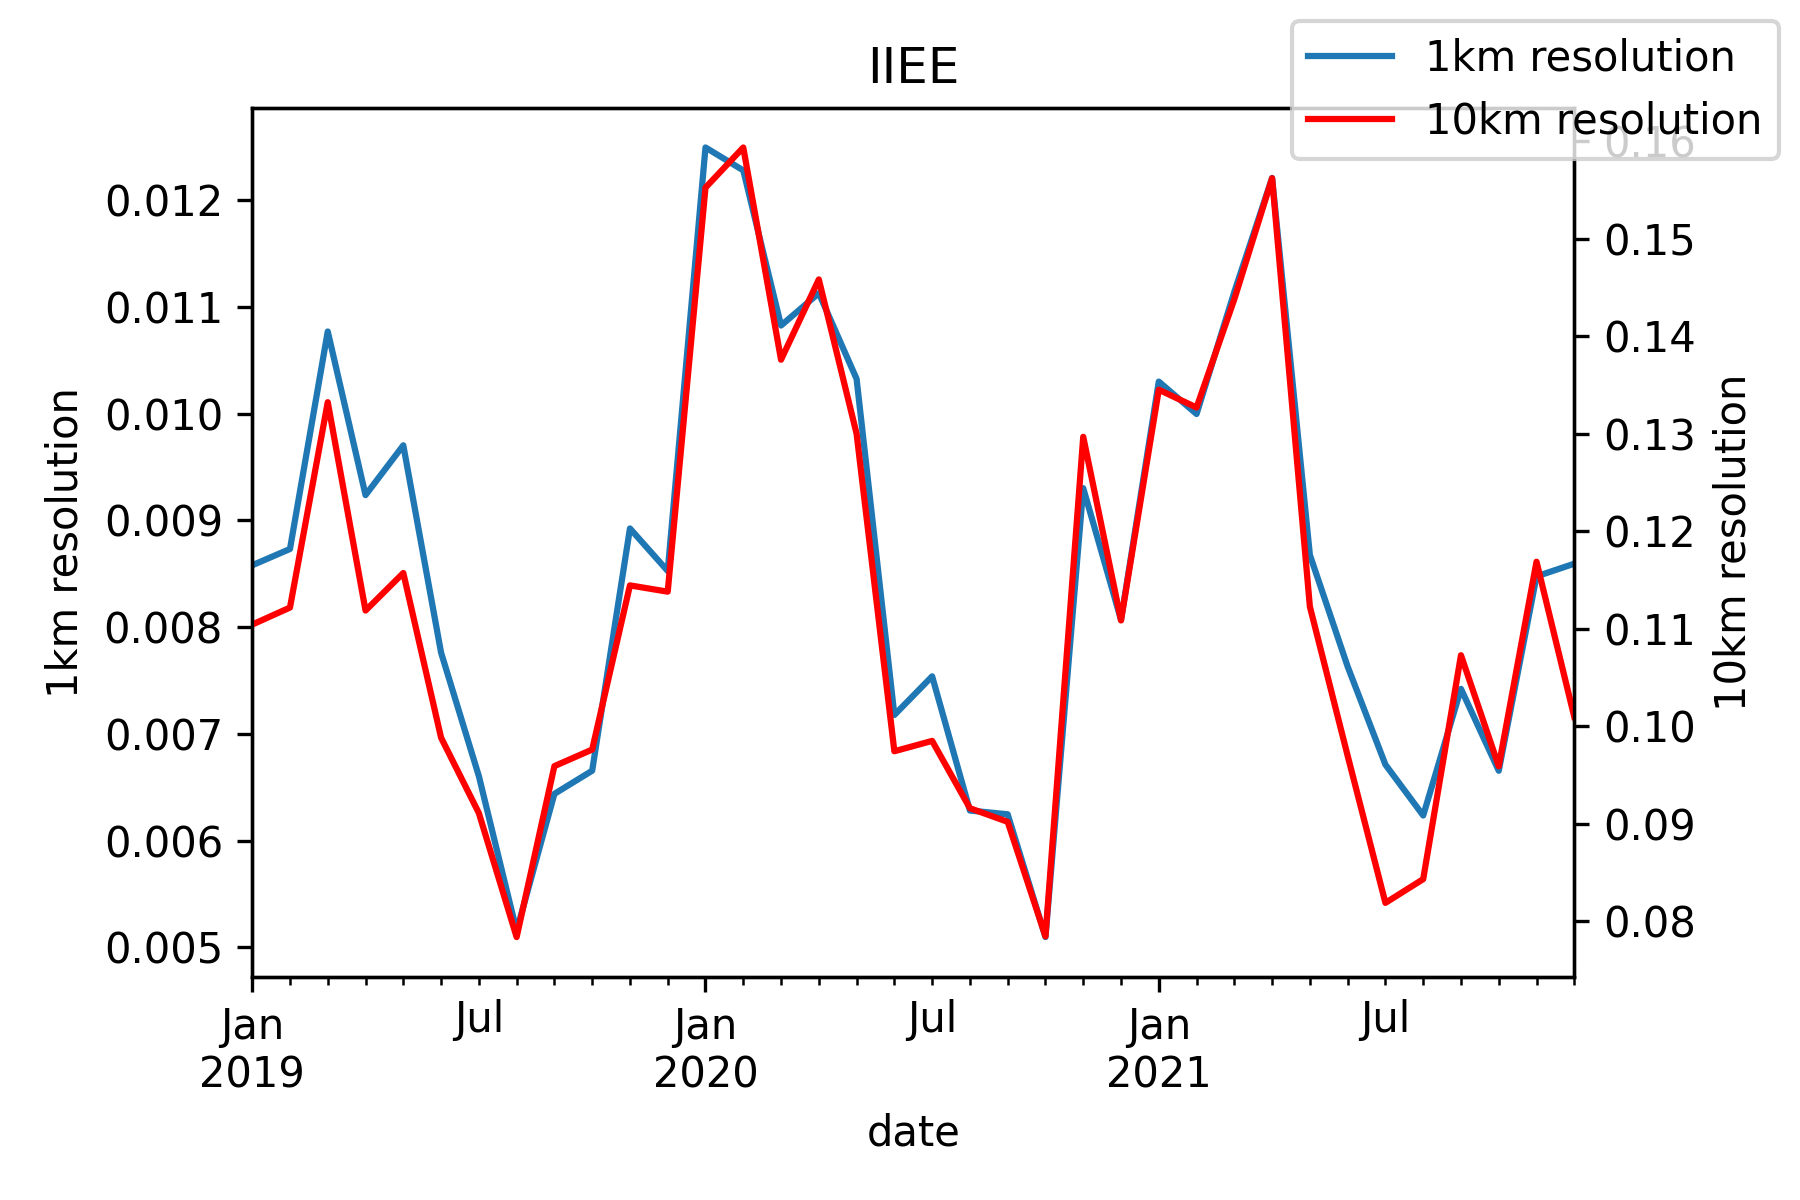
\includegraphics[width=\textwidth]{/home/arefk/uio/MScThesis_AreKvanum2022_SeaIceML/thesis/verification_metrics/figures/normalized_iiee.png}

    \caption{\label{fig:normIIEE}Monthly mean of Normalized IIEE spanning 2019 - 2021}
\end{figure}

\subsection{Computing distances with regards to an Ice Edge}
For the scope of this thesis, the above defined set E will be subscripted with \textit{f} and \textit{t} which represents \textit{forecast} and \textit{target} respectively. Hence, $E_f$ is the set of pixels which constitutes the forecasted ice edge, with $E_t$ defined analogously. With this definition, the euclidean displacement of the target ice edge $E_t$ from all forecasted ice grid cells $E_f$ has been defined as the following in \cite{Melsom2019}

\begin{equation}
    \label{eq:ice_edge_displacement}
    d_t^n = \min{\left(\forall e_f\in E_f : \left[(x_f - x_t^n)^2 + (y_f - y_t^n)^2\right]^{\frac{1}{2}}\right)}
\end{equation}

where x and y represent the coordinates of the grid cells and n the index of the pixel inspected in $E_t$. The opposite definition, i.e. the euclidean displacement of the forecasted ice edge in terms of the target ice edge is defined equally.

Equation (\ref{eq:ice_edge_displacement}) can also be generalized to hold for other use cases, not only comparing the displacement of two ice edges. Given an IIEE which has been separated into $A^+$ and $A^-$, and a target ice edge $E_t$, the distance between the nearest ice edge pixel $e_t$ two a misclassified pixel ($a^+$ or $a^-$) can be defined as, (using $a_+$ as an example)

\begin{equation}
    d_n = \min{\left(\forall e_t \in E_t : \text{distance($e_t$, $a_n^+$)}\right)}
\end{equation}

where distance is used to define som arbitrary distance metric, n denotes the pixel index in $A^+$. 

\biblio
\end{document}